% Options for packages loaded elsewhere
\PassOptionsToPackage{unicode}{hyperref}
\PassOptionsToPackage{hyphens}{url}
\PassOptionsToPackage{dvipsnames,svgnames,x11names}{xcolor}
%
\documentclass[
  letterpaper,
  DIV=11,
  numbers=noendperiod]{scrartcl}

\usepackage{amsmath,amssymb}
\usepackage{iftex}
\ifPDFTeX
  \usepackage[T1]{fontenc}
  \usepackage[utf8]{inputenc}
  \usepackage{textcomp} % provide euro and other symbols
\else % if luatex or xetex
  \usepackage{unicode-math}
  \defaultfontfeatures{Scale=MatchLowercase}
  \defaultfontfeatures[\rmfamily]{Ligatures=TeX,Scale=1}
\fi
\usepackage{lmodern}
\ifPDFTeX\else  
    % xetex/luatex font selection
\fi
% Use upquote if available, for straight quotes in verbatim environments
\IfFileExists{upquote.sty}{\usepackage{upquote}}{}
\IfFileExists{microtype.sty}{% use microtype if available
  \usepackage[]{microtype}
  \UseMicrotypeSet[protrusion]{basicmath} % disable protrusion for tt fonts
}{}
\makeatletter
\@ifundefined{KOMAClassName}{% if non-KOMA class
  \IfFileExists{parskip.sty}{%
    \usepackage{parskip}
  }{% else
    \setlength{\parindent}{0pt}
    \setlength{\parskip}{6pt plus 2pt minus 1pt}}
}{% if KOMA class
  \KOMAoptions{parskip=half}}
\makeatother
\usepackage{xcolor}
\setlength{\emergencystretch}{3em} % prevent overfull lines
\setcounter{secnumdepth}{-\maxdimen} % remove section numbering
% Make \paragraph and \subparagraph free-standing
\ifx\paragraph\undefined\else
  \let\oldparagraph\paragraph
  \renewcommand{\paragraph}[1]{\oldparagraph{#1}\mbox{}}
\fi
\ifx\subparagraph\undefined\else
  \let\oldsubparagraph\subparagraph
  \renewcommand{\subparagraph}[1]{\oldsubparagraph{#1}\mbox{}}
\fi


\providecommand{\tightlist}{%
  \setlength{\itemsep}{0pt}\setlength{\parskip}{0pt}}\usepackage{longtable,booktabs,array}
\usepackage{calc} % for calculating minipage widths
% Correct order of tables after \paragraph or \subparagraph
\usepackage{etoolbox}
\makeatletter
\patchcmd\longtable{\par}{\if@noskipsec\mbox{}\fi\par}{}{}
\makeatother
% Allow footnotes in longtable head/foot
\IfFileExists{footnotehyper.sty}{\usepackage{footnotehyper}}{\usepackage{footnote}}
\makesavenoteenv{longtable}
\usepackage{graphicx}
\makeatletter
\def\maxwidth{\ifdim\Gin@nat@width>\linewidth\linewidth\else\Gin@nat@width\fi}
\def\maxheight{\ifdim\Gin@nat@height>\textheight\textheight\else\Gin@nat@height\fi}
\makeatother
% Scale images if necessary, so that they will not overflow the page
% margins by default, and it is still possible to overwrite the defaults
% using explicit options in \includegraphics[width, height, ...]{}
\setkeys{Gin}{width=\maxwidth,height=\maxheight,keepaspectratio}
% Set default figure placement to htbp
\makeatletter
\def\fps@figure{htbp}
\makeatother

\KOMAoption{captions}{tableheading}
\makeatletter
\@ifpackageloaded{caption}{}{\usepackage{caption}}
\AtBeginDocument{%
\ifdefined\contentsname
  \renewcommand*\contentsname{Table of contents}
\else
  \newcommand\contentsname{Table of contents}
\fi
\ifdefined\listfigurename
  \renewcommand*\listfigurename{List of Figures}
\else
  \newcommand\listfigurename{List of Figures}
\fi
\ifdefined\listtablename
  \renewcommand*\listtablename{List of Tables}
\else
  \newcommand\listtablename{List of Tables}
\fi
\ifdefined\figurename
  \renewcommand*\figurename{Figure}
\else
  \newcommand\figurename{Figure}
\fi
\ifdefined\tablename
  \renewcommand*\tablename{Table}
\else
  \newcommand\tablename{Table}
\fi
}
\@ifpackageloaded{float}{}{\usepackage{float}}
\floatstyle{ruled}
\@ifundefined{c@chapter}{\newfloat{codelisting}{h}{lop}}{\newfloat{codelisting}{h}{lop}[chapter]}
\floatname{codelisting}{Listing}
\newcommand*\listoflistings{\listof{codelisting}{List of Listings}}
\makeatother
\makeatletter
\makeatother
\makeatletter
\@ifpackageloaded{caption}{}{\usepackage{caption}}
\@ifpackageloaded{subcaption}{}{\usepackage{subcaption}}
\makeatother
\ifLuaTeX
  \usepackage{selnolig}  % disable illegal ligatures
\fi
\usepackage{bookmark}

\IfFileExists{xurl.sty}{\usepackage{xurl}}{} % add URL line breaks if available
\urlstyle{same} % disable monospaced font for URLs
\hypersetup{
  pdftitle={Physical activity as an effect modificator of lifestyle factors on small vessel deisease burden},
  colorlinks=true,
  linkcolor={blue},
  filecolor={Maroon},
  citecolor={Blue},
  urlcolor={Blue},
  pdfcreator={LaTeX via pandoc}}

\title{Physical activity as an effect modificator of lifestyle factors
on small vessel deisease burden}
\author{Andreas Gammelgaard Damsbo \and Rolf Ankerlund
Blauenfeldt \and Grethe Andersen \and Janne Kaergaard Mortensen}
\date{}

\begin{document}
\maketitle
\begin{abstract}
\textbf{Background and aims} Physical activity (PA) may reduce the
development of small vessel disease (SVD). The effect of physical
activity and more classical vascular risk factors such as hypertension
and diabetes in the development of SVD is debated, however. We aim to
investigate the effect modification of physical activity on traditional
vascular risk factors and the burden of small vessel disease among acute
ischemic stroke patients.

\textbf{Methods} We have pooled patients from two clinical trials on
acute ischemic stroke treatment. The main outcome is an ordinal scale
score of quantified MR biomarkers of small vessel disease (SVD) burden
based on visually assessed acute stroke scans (T2* or SWI and FLAIR
sequences). Biomarkers includes microbleeds, old lacunar infarcts,
superficial siderosis, white matter hyperintensities and atrophy.
Covariates includes age, sex, pre-stroke physical activity, diabetes,
hypertension, atrial fibrillation and previous cardiovascular diseases.
Pre-stroke PA was assessed with a questionnaire on inclusion within a
few days after stroke onset. Data will be analyzed using bivariate and
multivariate linear regression analysis.

\textbf{Results} We expect to include a total of around 1000 adult
patients admitted to the comprehensive stroke centre at Aarhus
University Hospital between 2013-2022. Preliminary results will be
presented at ESOC 2024.

\textbf{Conclusions} Physical activity may be an important factor in
modifying the risk of SVD development in stroke patients.
\end{abstract}

\textsubscript{Source:
\href{https://agdamsbo.github.io/svd-modification/index.qmd.html}{Article
Notebook}}

\subsection{Introduction}\label{introduction}

This is, for now, just a placeholder for upcoming article on physical
activity as an effect modificator of lifestyle factors on the burden of
small vessel disease in stroke patients.

\subsection{Methods}\label{methods}

This study is based on a pooled dataset from two different randomised,
clinical trials on stroke patients.

\subsection{Results}\label{results}

Please refer to Figure~\ref{fig-flowchart} for an overview of subjects
included for analysis.

\begin{figure}

\centering{

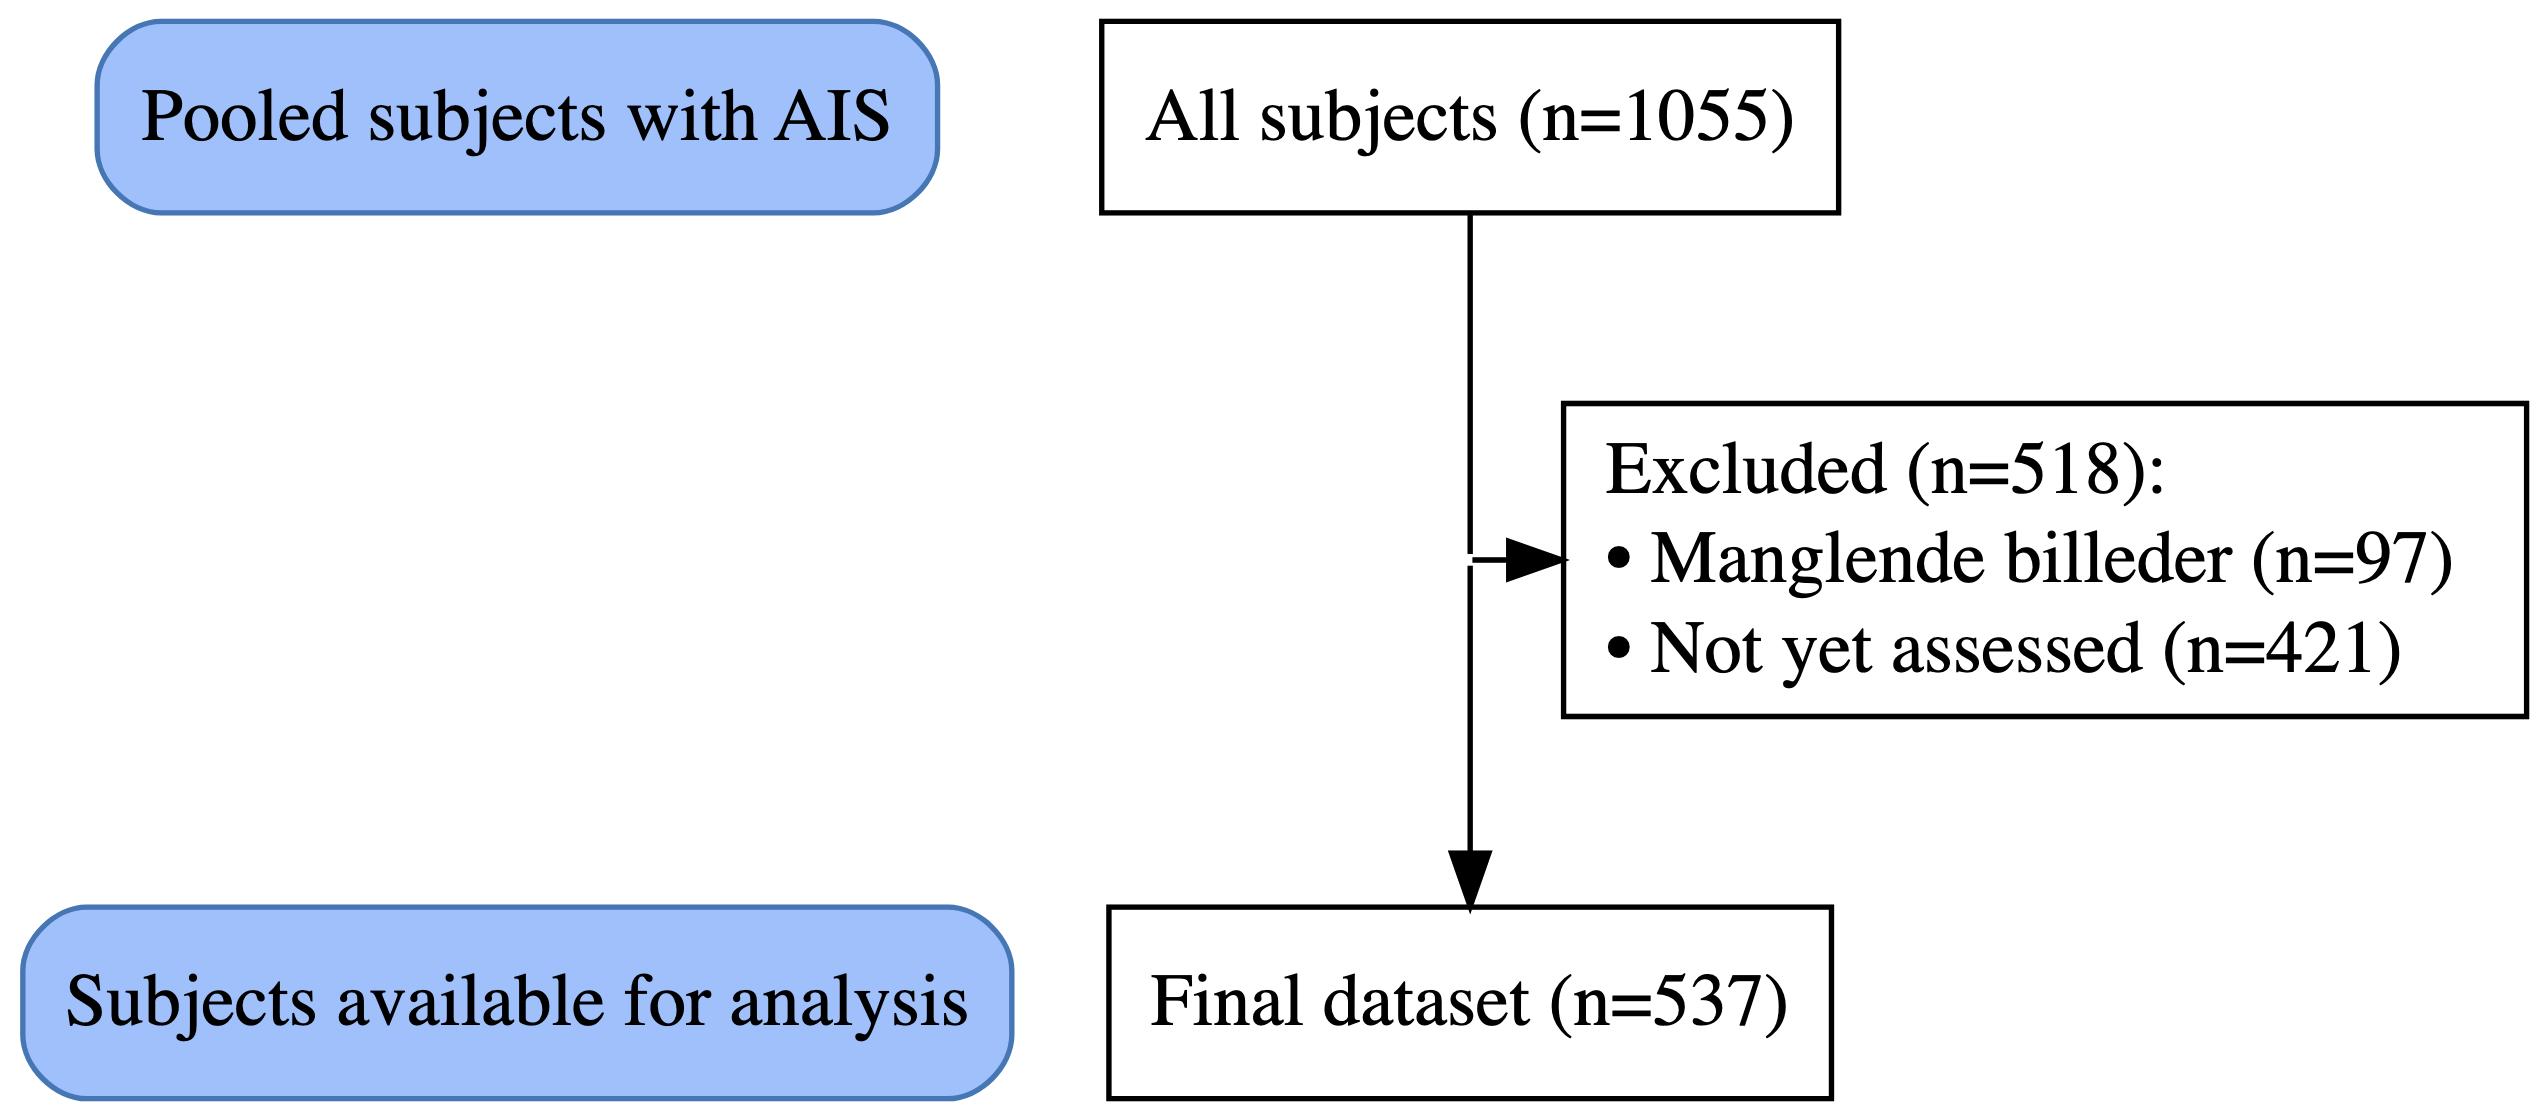
\includegraphics[width=5.5in,height=3.5in]{index_files/figure-latex/dot-figure-2.png}

}

\caption{\label{fig-flowchart}Flowchart of subject included for
analysis}

\end{figure}%

\textsubscript{Source:
\href{https://agdamsbo.github.io/svd-modification/index.qmd.html}{Article
Notebook}}



\end{document}
